\documentclass{beamer}
\usetheme{CambridgeUS}
\usecolortheme{dolphin} 
\usepackage[utf8]{inputenc}
\usepackage[spanish]{babel}
\usepackage{graphicx}


\title[Tecnologia]
{Algoritmo incorrecto de Hyman}
\subtitle{}
\author[Grupo 1] 
{Ignacio P\'erez Laborda\\B\'arbara Mart\'inez}
\institute[UB--FTI] 
{
  Facultad de Tecnolog\'ia Inform\'atica\\
  Universidad de Belgrano
}
\date[\today] 

\renewcommand{\thefootnote}{\roman{footnote}}

\begin{document}
%1
%\frame{\titlepage}

\begin{frame}


\includegraphics[height=0.2\textheight]{ub2.jpg} \hspace*{6cm}

\includegraphics[height=0.19\textheight]{FTI.jpg}  
\\[-0.1cm]
\titlepage


\end{frame}

\begin{frame}{Introducción}
\begin{enumerate}
\item Este algoritmo se penso para darle una solucion al problema de la exclusion mutua en la programación concurrente.
\item  Harris Hyman, estudiante universitario, propuso esta solucion en 1966 basandose en el existente algoritmo de petersen.
\item Fue publicado en un diario escolar pero luego los publicantes se retractaron debido a que luego descubrieron que  el algoritmo era incorrecto.
\end{enumerate}

\end{frame}

\begin{frame}[fragile]

\frametitle{Código fuente del Algoritmo} \vspace*{-0.8 cm}
	\begin{verbatim}

void Protocol (int me, int you)
{
        do 
        {
1.        flag[me] = true ;
2.        while (turn != me)
          {
3.             while (flag[you])
4.               /* do nothing */ ;
5.             turn = me
          }
6.        CriticalSection(me) ;
7.        flag[me] = false ;
8.        RemainderSection(me) ;
        } while (true) ;
}

	\end{verbatim}

\end{frame}

\begin{frame}
\frametitle{Descripción} 

 Consiste en turnar la ejecución de dos procesos concurrentes , cuando uno esta trabajando , ciclará hasta que termine y luego pasará al proceso siguiente.\par
Sin embargo el algoritmo presenta fallas en la resolución de la exclusion mutua.A Continuación mostraremos un ejemplo en el cual falla.
%ampliar 
\end{frame}


\begin{frame}
\frametitle{Ejemplo} 
Supongamos que:
\begin {enumerate}[$*$]
\item La variable turn esta en 0 
\item Los flags[0] y flags[1] estan en falso
\item Los procesos a ejecutar son 1,2,3,5 y 6
\end{enumerate}
 El proceso P1 ejecuta 1,2,3 . Como flag[0] es falso , la proxima instruccion que debe ejecutar P1 seria 5, pero lo hara proximamente.\par
 P0 ejecuta 1,2 y 6.\par
Y por ultimo P0 quiere ejecutar 5 y 6 pero no puede porque P0 está trabajando en el proceso 6, ambos se encuentran en la exclusión mutua.

\end{frame}

\begin{frame}
\frametitle{Ejemplo} 
Esta es una imagen demostrativa de la ejecución del algoritmo \vspace*{0.3cm}

 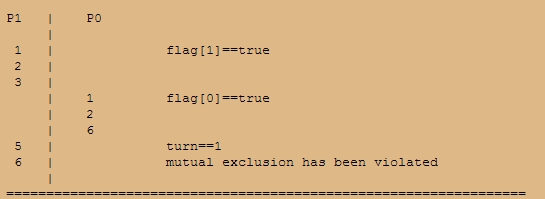
\includegraphics[width=1\textwidth]{scenario.png}


\end{frame}

\end{document}

